\chapter{LHC Data for Parton Determinations}
\label{ch:LHCdata}
The Large Hadron Collider has the ability to provide a comprehensive examination of QCD and electroweak physics at a wide range of scales. The requirement of precise and reliable
determinations of proton structure is clear in order to fully exploit the LHC's potential. LHC data also has the potential to provide deep new insights into parton distributions, examining hitherto
poorly determined flavours and kinematic regimes. A great deal of effort has therefore been expended in providing and validating tools for the inclusion of LHC data in an efficient manner into
NNPDF fits.

In this section the Standard Model measurements of relevance to PDF determination so far performed by the LHC shall be briefly summarised. While the general processes have been described previously,
here we shall look directly at the experimental data along with a brief examination of the areas of agreement or discrepancy with regard to PDF sets made available before the first data runs of the LHC.

\section{Jet measurements}
At the LHC, data on the production of collimated jets of particles originating from partonic final states provides valuable information on proton structure and additional constraints for $\alpha_S$ determinations. The LHC's centre-of-mass energies
mean that jets with transverse momenta in the TeV range are observable for the first time. Forward jets probing the very large-$x$ gluon that has suffered from poor constraints prior to the LHC. As the prototypical QCD measurement, data
is available from both of the general purpose LHC experiments, and preliminary data on jets in the forward region is available from LHCb~\cite{LHCb:2011xqa}. LHC measurements are based upon modern infrared and collinear safe jet-finding algorithms such as anti-$k_T$~\cite{Cacciari:2008gp}. In PDF fits the jet quantity of interest is typically the inclusive measurement rather than dijet data. In principle dijet measurements offer more discriminating power over the parton distributions, however they typically suffer from larger scale uncertainties and often must be corrected for higher order effects, typically modelled through parton showers.

 Here we shall summarise the relevant jet measurements at the LHC with a focus on the data most relevant to PDF determination.

The first ATLAS inclusive jet and dijet measurements were based upon a partial analysis of $17$ nb$^{-1}$ of data available from the 2010 data run at a centre of mass energy of $7$ TeV~\cite{Aad:2010ad}. This result was then updated to the full 2010 dataset of $37$ pb$^{-1}$~\cite{Aad:2011fc}.
The full 2010 measurement presents the inclusive jet cross section differentially in both the jet $p_T$ and rapidity. Data is available for the $20 \le p_T < 1500$ GeV range for jets with rapidity $|y|<4.4$, and is available for two choices of the anti-$k_T$ cone size, $R=0.4$ and $R=0.6$.
\begin{figure}[ht]
\centering
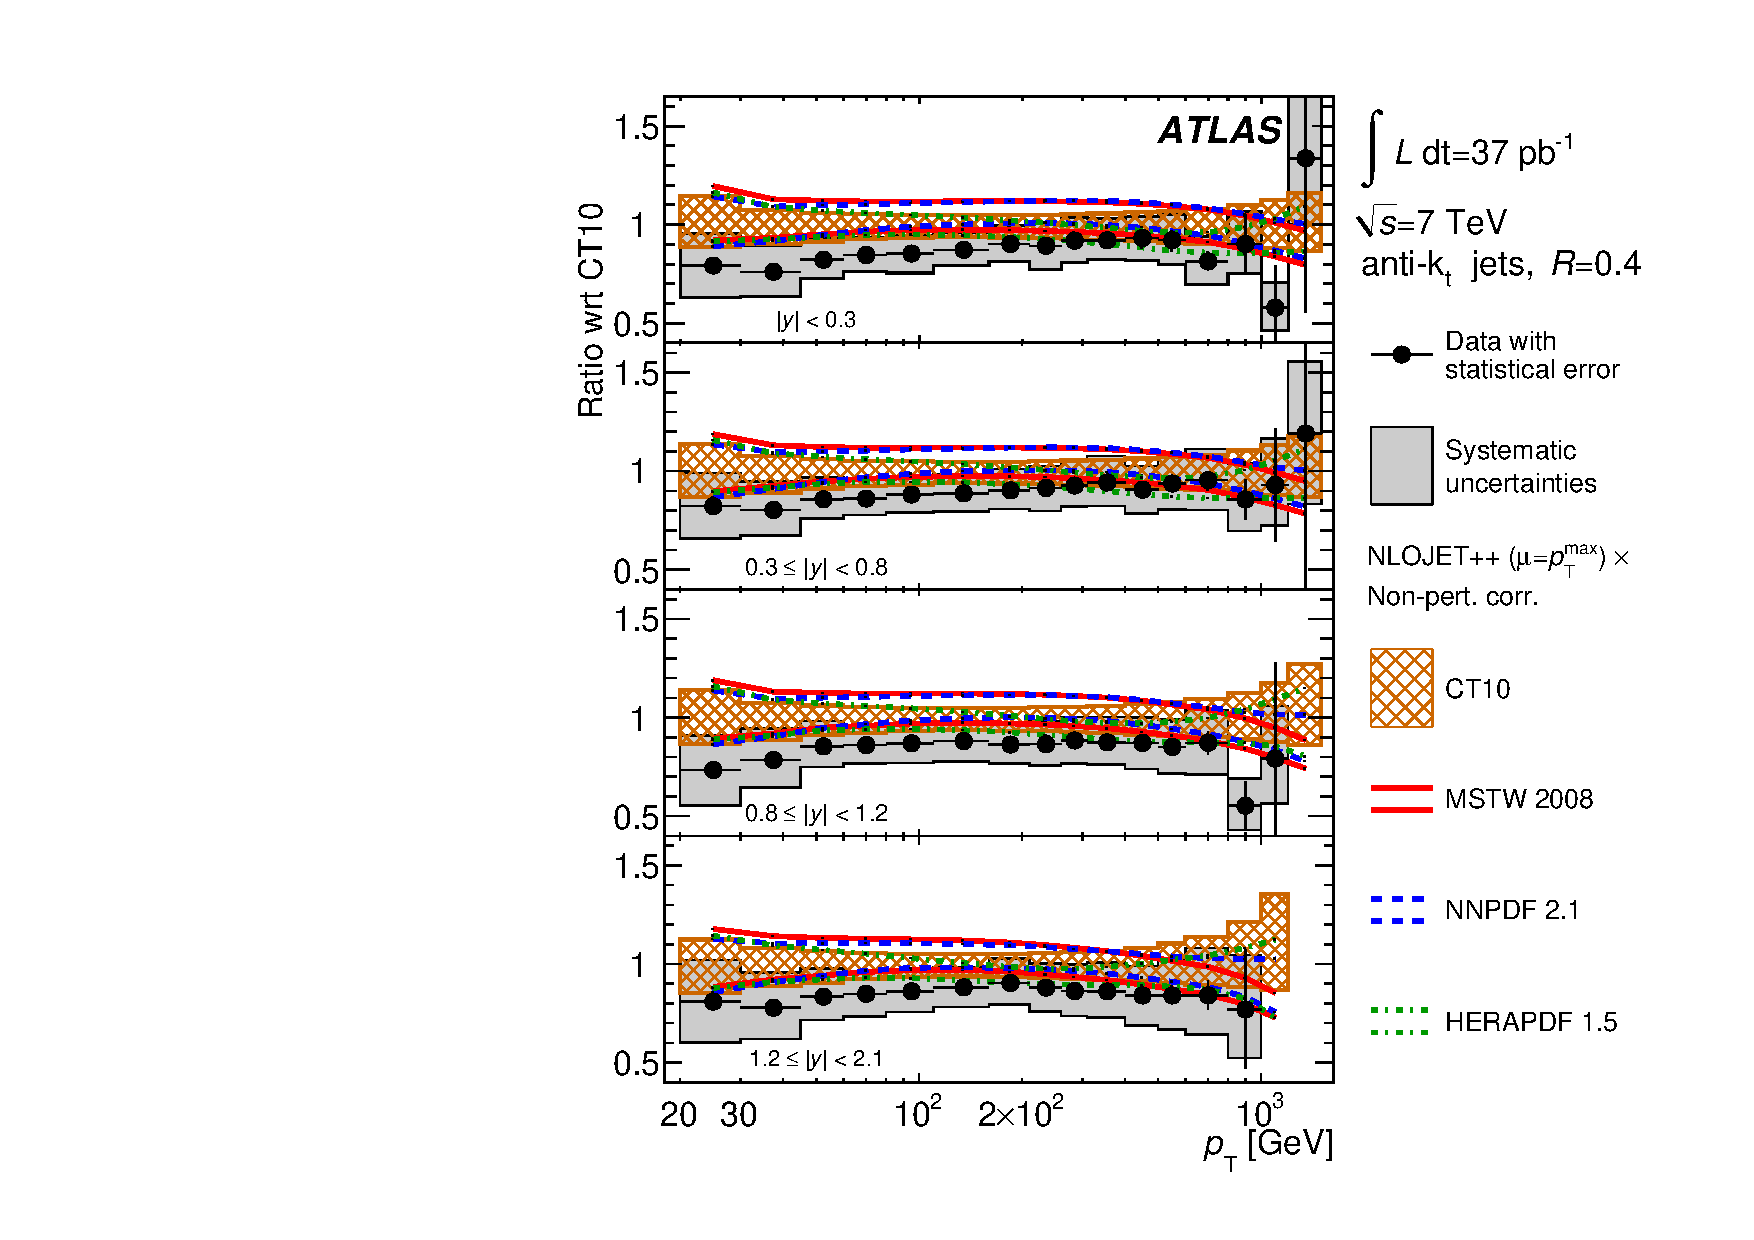
\includegraphics[width=0.48\textwidth]{5-LHCdata/figs/fig_12a.pdf}
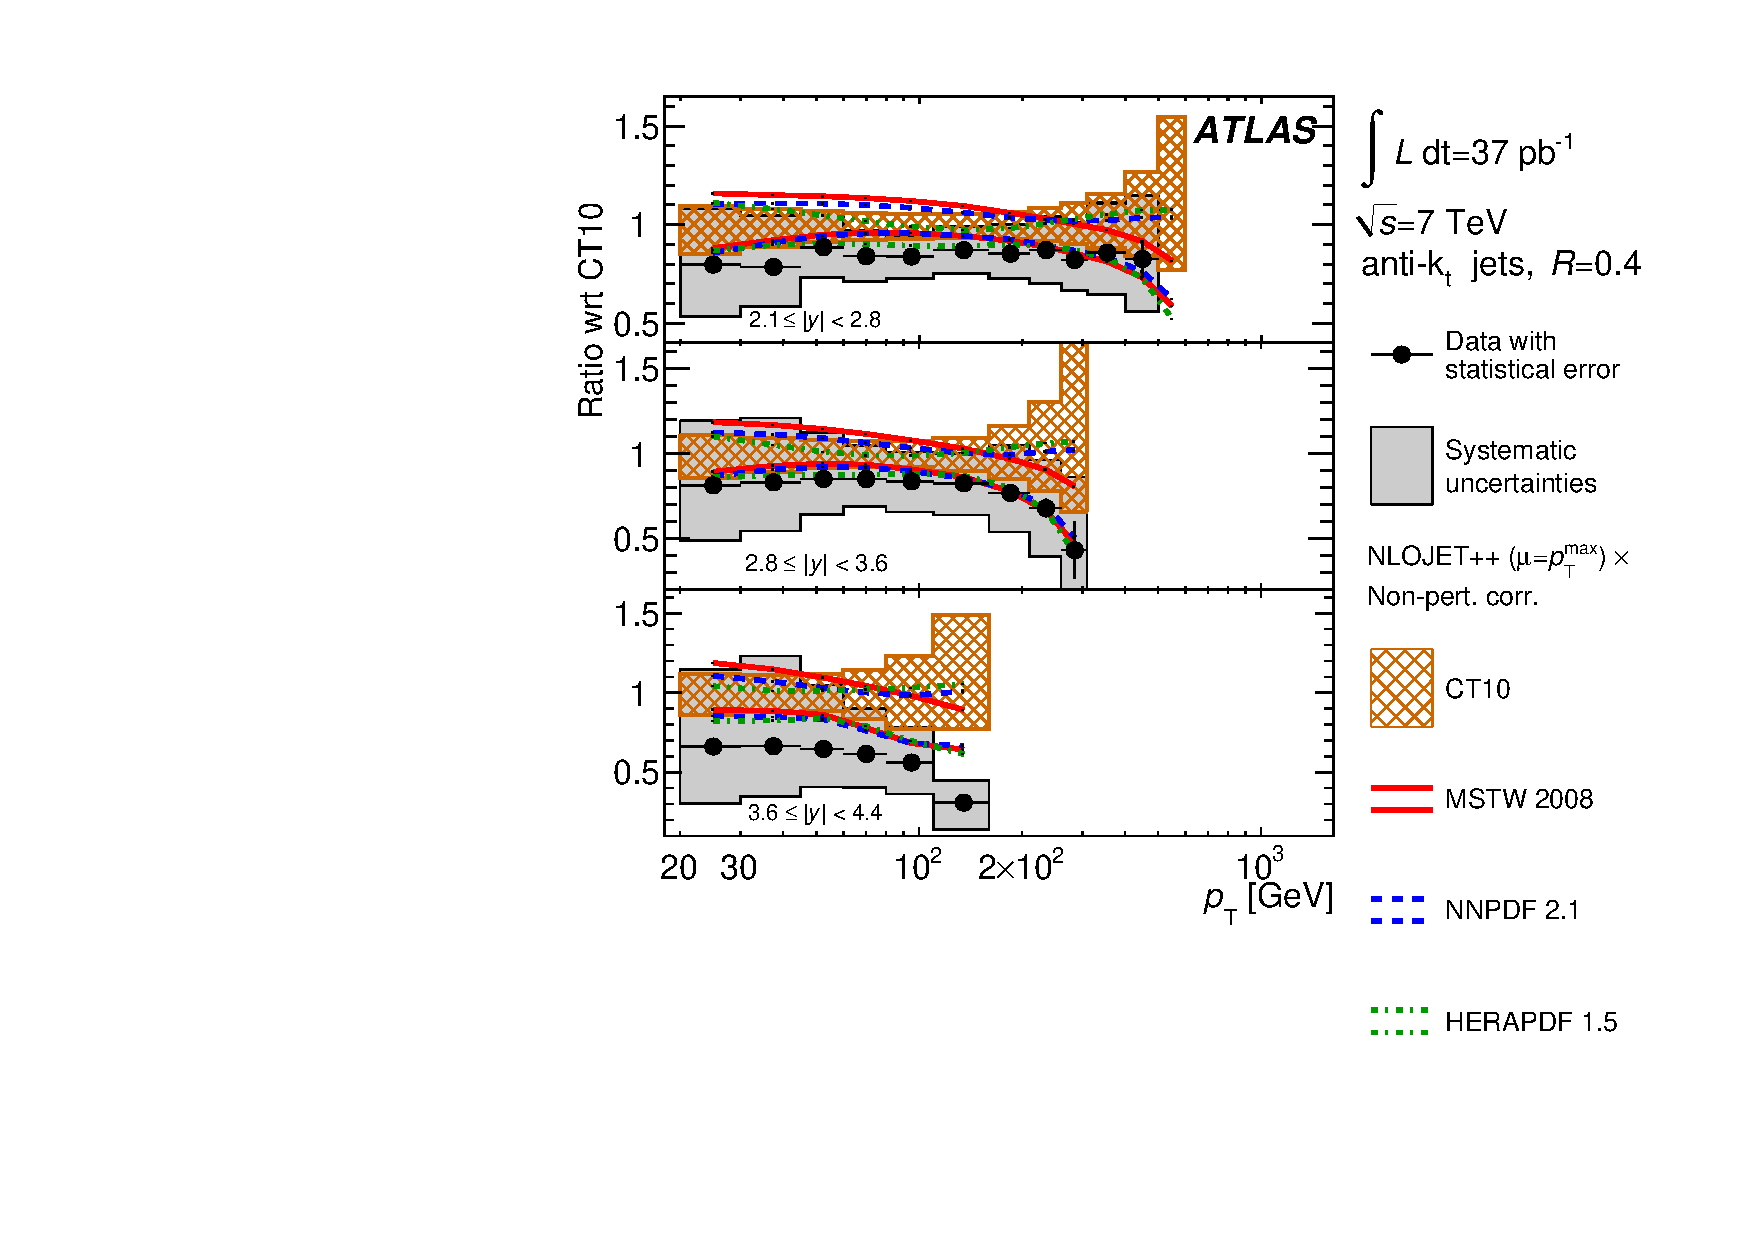
\includegraphics[width=0.48\textwidth]{5-LHCdata/figs/fig_12b.pdf}
\caption[ATLAS inclusive jet data with anti-$k_T$ algorithm $R=0.4$]{ATLAS inclusive jet data with anti-$k_T$ algorithm $R=0.4$ from the 2010 dataset. Figures from~\cite{Aad:2011fc}. Predictions are shown based upon MSTW2008, NNPDF2.1 and HERAPDF1.5 PDFs, with all data and theory normalised to the CT10 central value.}
\label{fig:ATLASR04Jets}
\end{figure}

Figure~\ref{fig:ATLASR04Jets} from the ATLAS $37$ pb$^{-1}$ result demonstrates the level of agreement of the fixed-order NLO inclusive jet computation present in {\tt NLOJet++} with the experimental data given four choices of PDFs: CT10, MSTW2008, NNPDF2.1 and HERAPDF1.5. Predictions from the four sets largely agree within their PDF uncertainties, and the experimental data also shows good agreement for most of the data range. Some evidence of a systematic discrepancy is visible at large $p_T$, an effect that becomes more noticeable in the larger rapidity bins (and therefore more extreme values of parton-$x$).  

ATLAS has also published data on the inclusive jet cross-sections at $\sqrt{s} = 2.76$ GeV measured during the 2011 run~\cite{Aad:2013lpa}. The data provides an important link between jet measurements at lower centre-of-mass energies at the Tevatron and the higher scale measurements previously published. In addition, the ratio of the $\sqrt{s} = 2.76$ GeV data to the 2010 $\sqrt{s}=7$ GeV measurement is presented. The ratio offers additional important constraints in that the dominant uncertainties upon the jet measurements are systematic across both datasets, and therefore largely cancel in the ratio. Figure~\ref{fig:ATLASJETSRAT} demonstrates the reduced uncertainty in the measurement, and therefore the additional constraint that the data may provide parton fits.

\begin{figure}[ht]
\centering
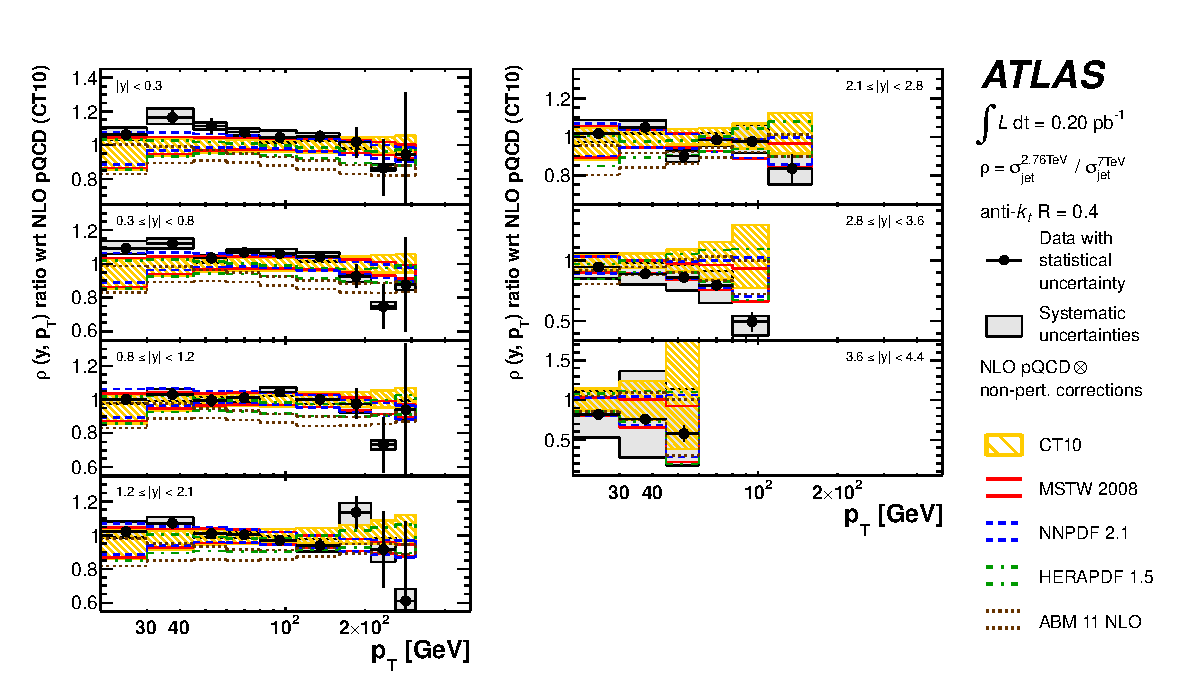
\includegraphics[width=0.90\textwidth]{5-LHCdata/figs/FinalRatioBandPTR04.pdf}
\caption[ATLAS inclusive jet ratio between $\sqrt{s} = 2.76$ GeV and $7$ GeV data] {ATLAS inclusive jet ratio between $\sqrt{s} = 2.76$ GeV and $7$ GeV data, anti-$k_T$ $R=0.4$. Figures from ~\cite{Aad:2013lpa}.}
\label{fig:ATLASJETSRAT}
\end{figure}


CMS has published three measurements of inclusive and dijet observables to date. The first provided data in the $18 < p_T < 1100$ GeV interval for jets with $|y|<3$ based upon $34$pb$^{-1}$ of 2010 data~\cite{CMS:2011ab}. This was followed up
by a study of jets in the forward region~\cite{Chatrchyan:2012gwa}, examining inclusive jets with pseudorapidities $3.2<|\eta|<4.7$, and dijets with one forward jet and one central $|\eta|<2.8$ jet. A study of 2011 data totalling $5.0$fb$^{-1}$ was also
performed of jets in the central $|y|<2.5$ region up to very high jet transverse momenta $p_T < 2$ TeV~\cite{Chatrchyan:2012bja}. CMS also utilises the anti-$k_T$ clustering algorithm, with cone sizes $R=0.5$ and $R=0.7$.


\begin{figure}[ht]
\centering
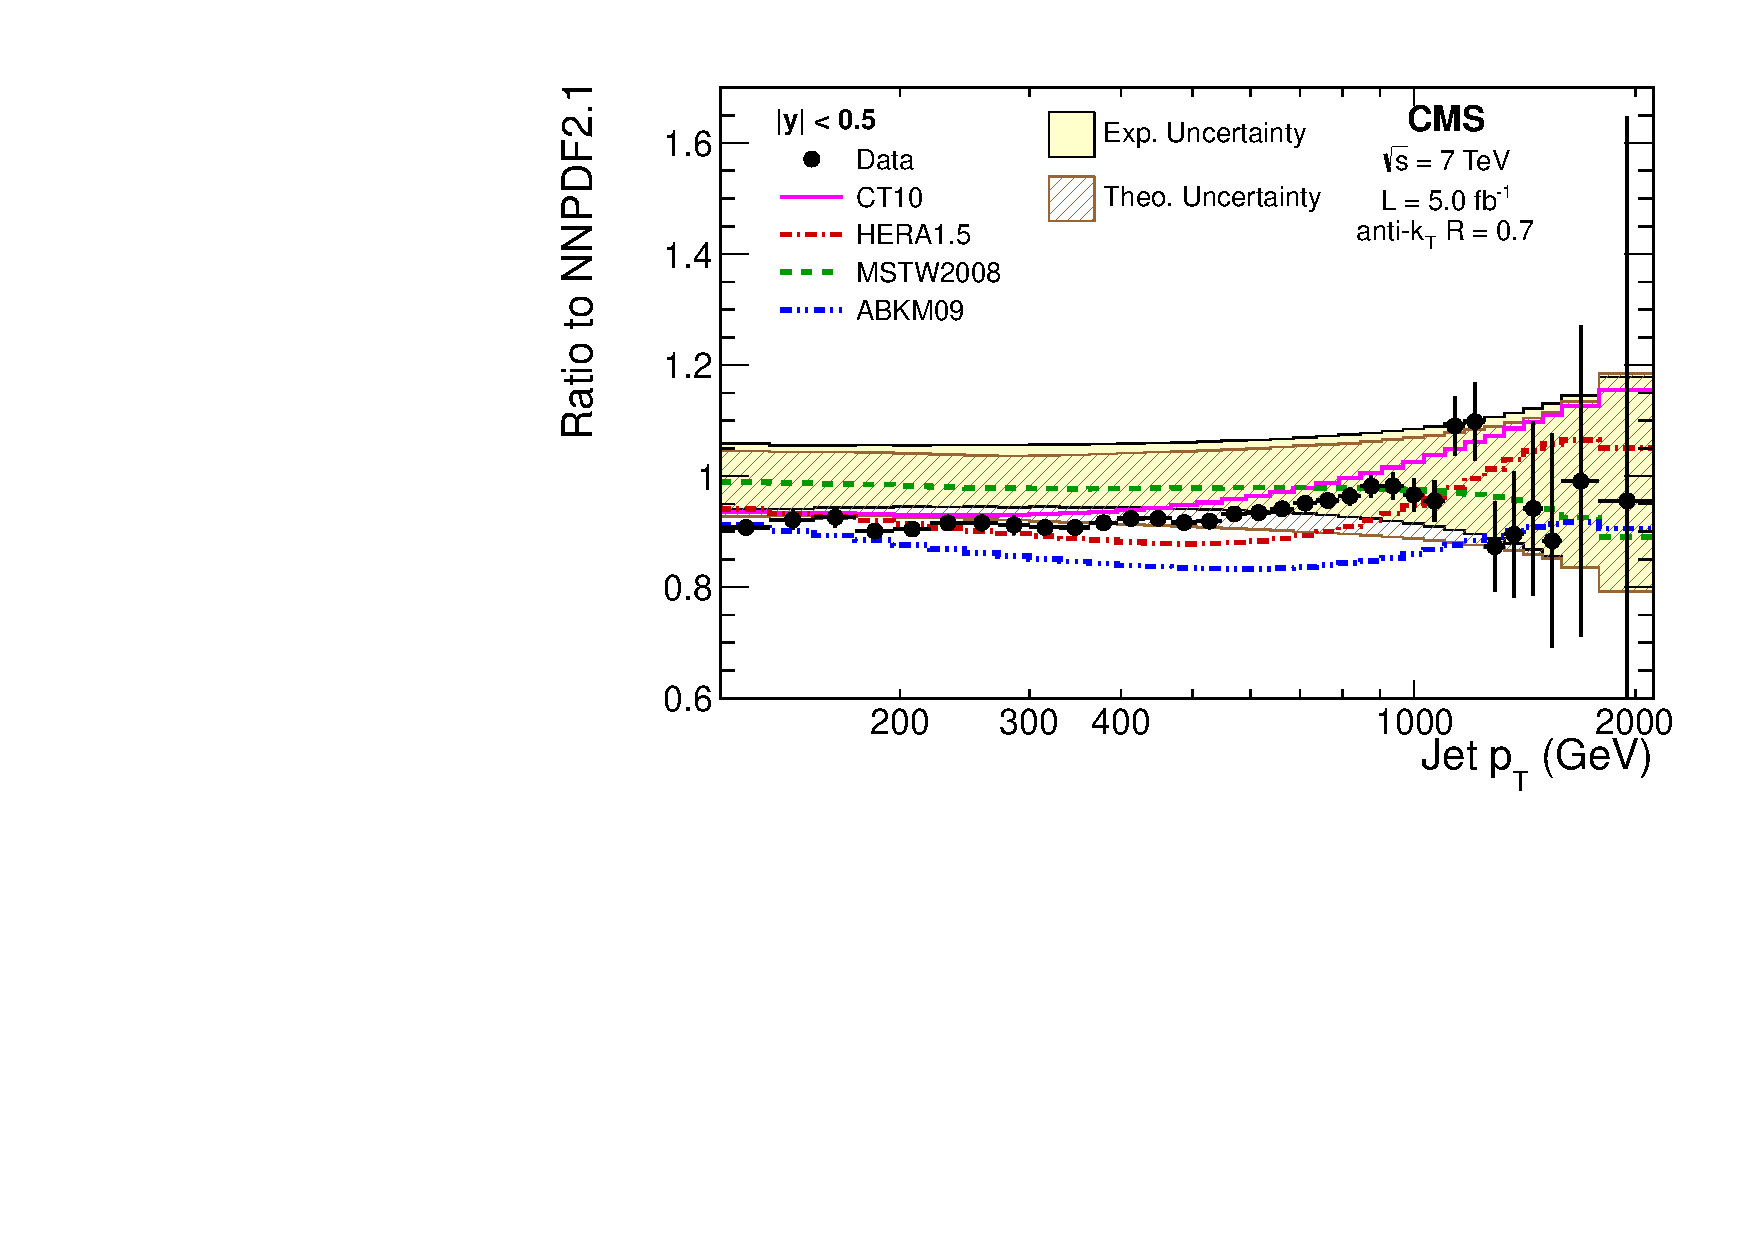
\includegraphics[width=0.48\textwidth]{5-LHCdata/figs/Inclusive_Data_over_Theory_Ybin0.pdf}
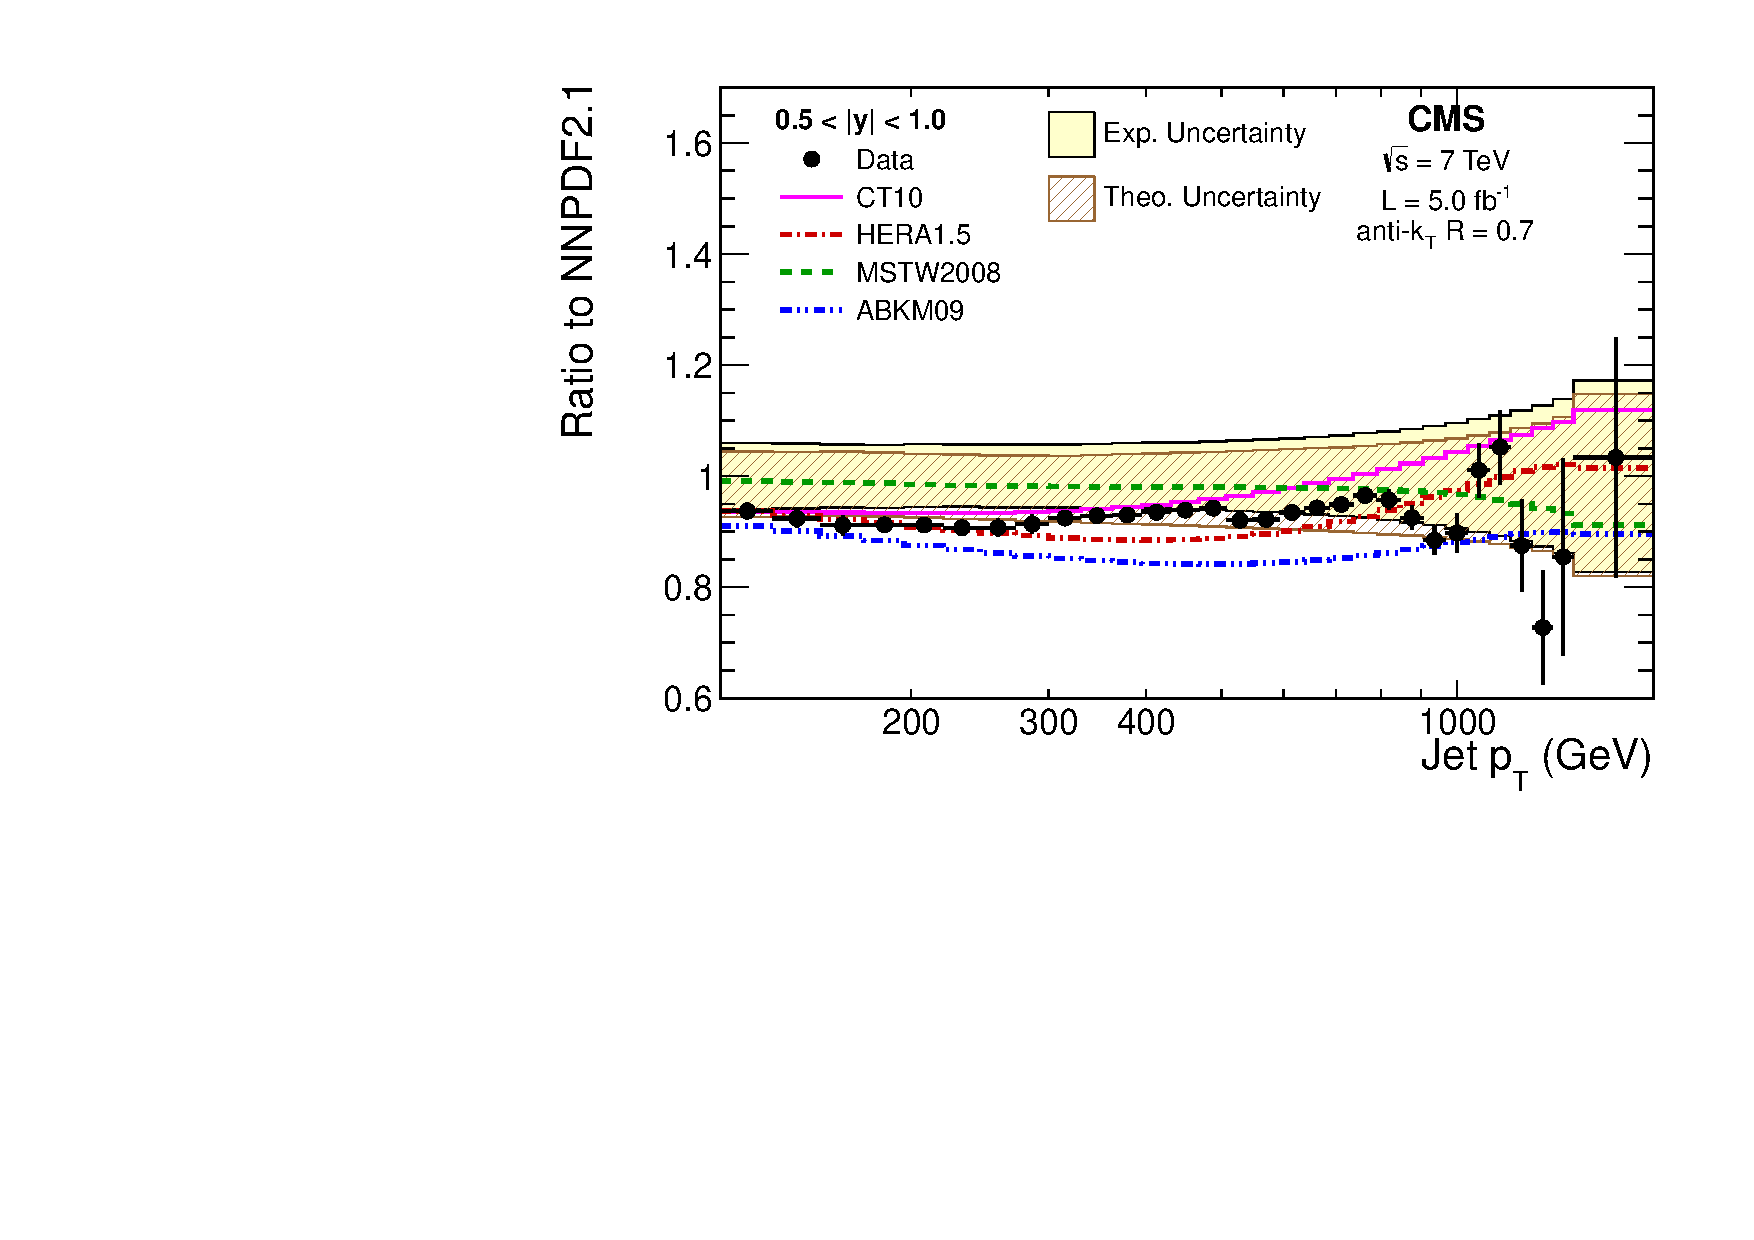
\includegraphics[width=0.48\textwidth]{5-LHCdata/figs/Inclusive_Data_over_Theory_Ybin1.pdf}
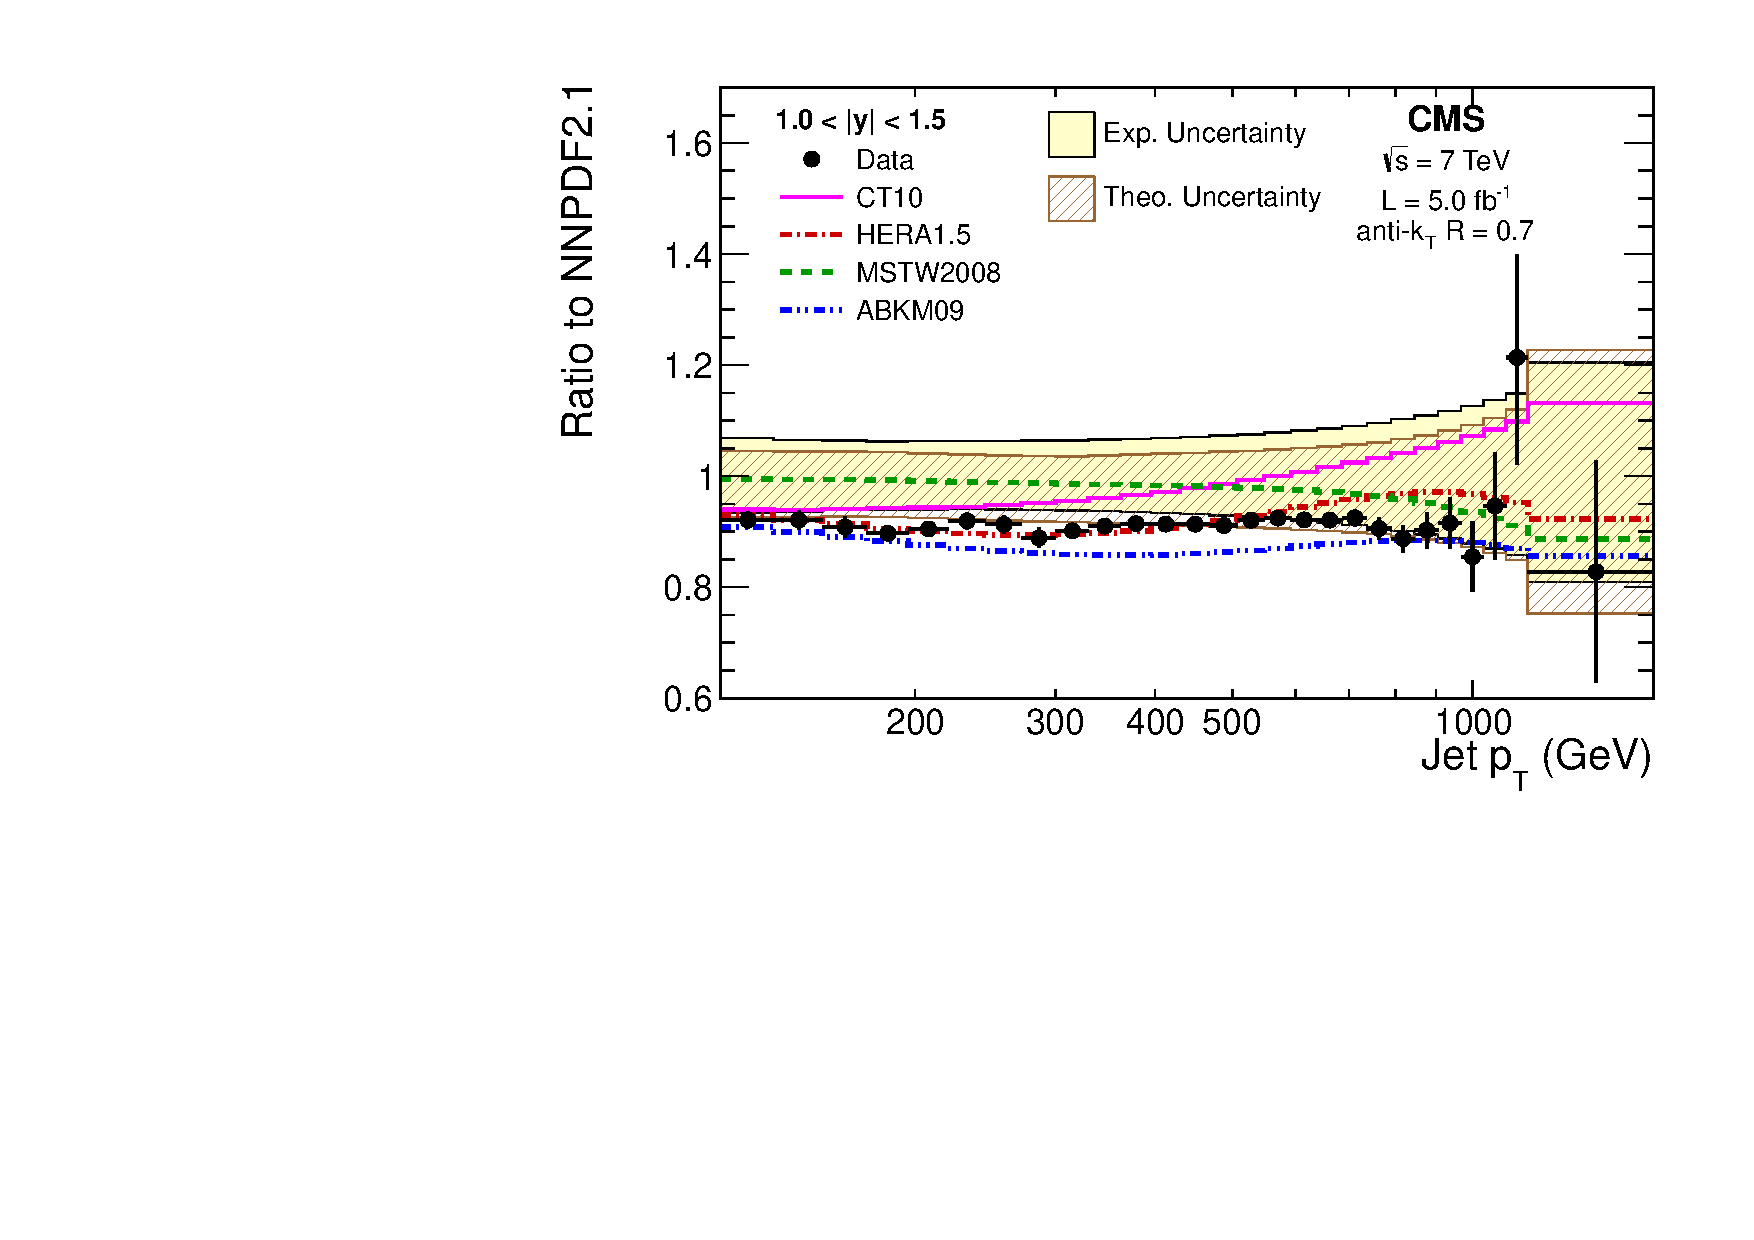
\includegraphics[width=0.48\textwidth]{5-LHCdata/figs/Inclusive_Data_over_Theory_Ybin2.pdf}
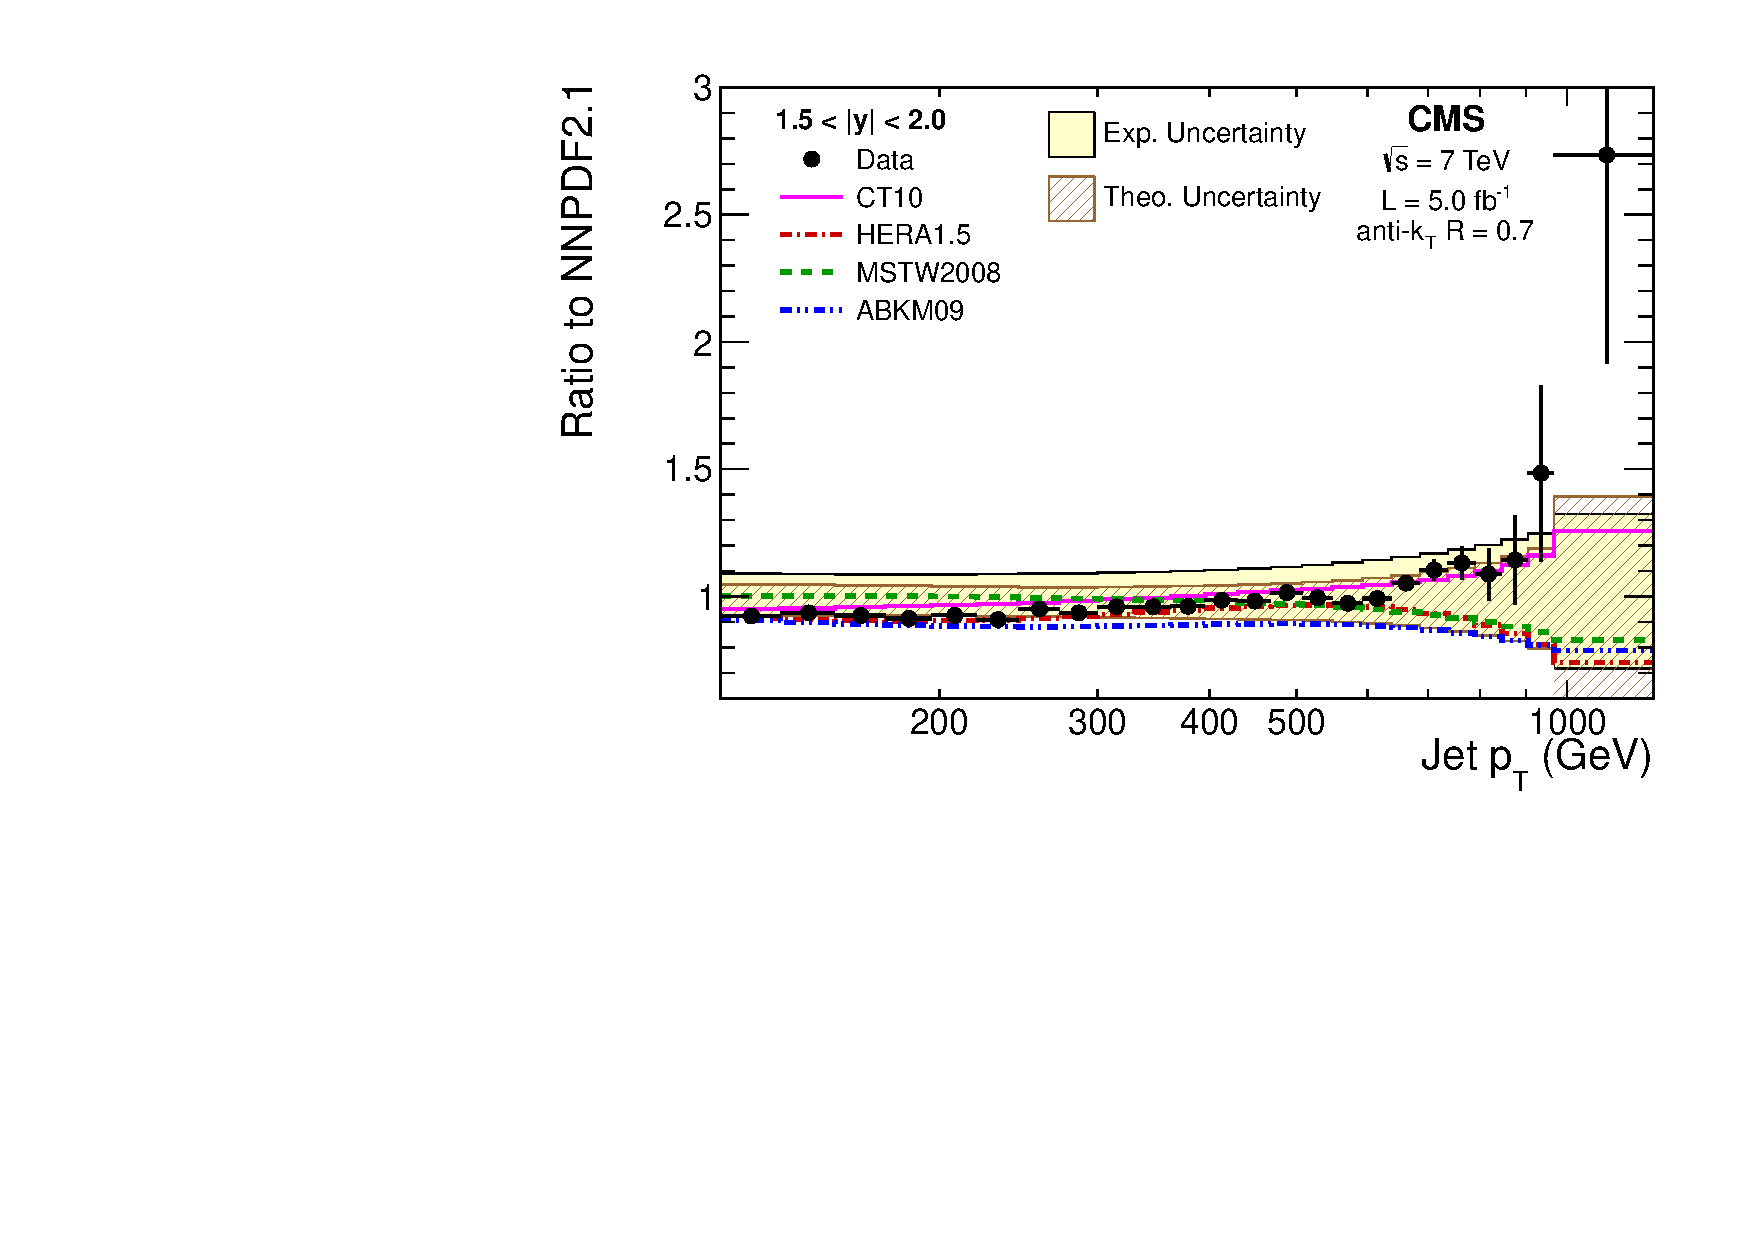
\includegraphics[width=0.48\textwidth]{5-LHCdata/figs/Inclusive_Data_over_Theory_Ybin3.pdf}
\caption[CMS inclusive jet data with anti-$k_T$ algorithm $R=0.7$]{CMS inclusive jet data with anti-$k_T$ algorithm $R=0.7$ from the 2011 dataset. Figures from~\cite{Chatrchyan:2012bja}. Predictions are shown based upon MSTW2008, NNPDF2.1 and HERAPDF1.5 PDFs, with all data and theory normalised to the NNPDF2.1 central value.}
\label{fig:CMSR07Jets}
\end{figure}

Figure~\ref{fig:CMSR07Jets} shows the inclusive data from the CMS central region jet measurement normalised to the NNPDF2.1 central value. Results are once again largely consistent with PDFs determined with pre-LHC data. 

%
%\begin{figure}[ht]
%\centering
%\includegraphics[width=0.48\textwidth]{5-LHCdata/figs/fig_16a.pdf}
%\includegraphics[width=0.48\textwidth]{5-LHCdata/figs/fig_16b.pdf}
%\caption[ATLAS dijet data with anti-$k_T$ algorithm $R=0.4$]{ATLAS dijet data with anti-$k_T$ algorithm $R=0.6$. Figures from ~\cite{Aad:2011fc}.}
%\label{fig:ATLASR06JETS}
%\end{figure}


\section{$W$/$Z$ boson production}

The measurement of electroweak vector boson production and Drell-Yan cross sections are standard candle measurements for the LHC, and have been widely studied by ATLAS, CMS and LHCb in the first run.

CMS has presented measurements of the $Z$ boson $p_T$ and rapidity distributions, initially upon $36$pb$^{-1}$ of $7$ TeV 2010 data~\cite{Chatrchyan:2011wt}, and more recently a preliminary
study of $8$ TeV data on Z decay to dimuons~\cite{CMS-PAS-SMP-12-025,CMS-PAS-SMP-13-013}. The first differential measurements of $W$ boson production at CMS were lepton charge asymmetry measurements
based upon 2010 data~\cite{Chatrchyan:2011jz}, which were superseded by the muon asymmetry measurement based upon $840$pb$^{-1}$, and then $4.6$pb$^{-1}$ of 2011 data~\cite{Chatrchyan:2012xt,Chatrchyan:2013mza}. In Figure~\ref{fig:CMS2010WASY}
the 2010 data $W$ asymmetry measurement of CMS is shown, demonstrating the constraining power of the earlier CMS result, where agreement is generally good with the pre-LHC parton distributions with the exception of the MSTW 2008 description.

\begin{figure}[ht]
\centering
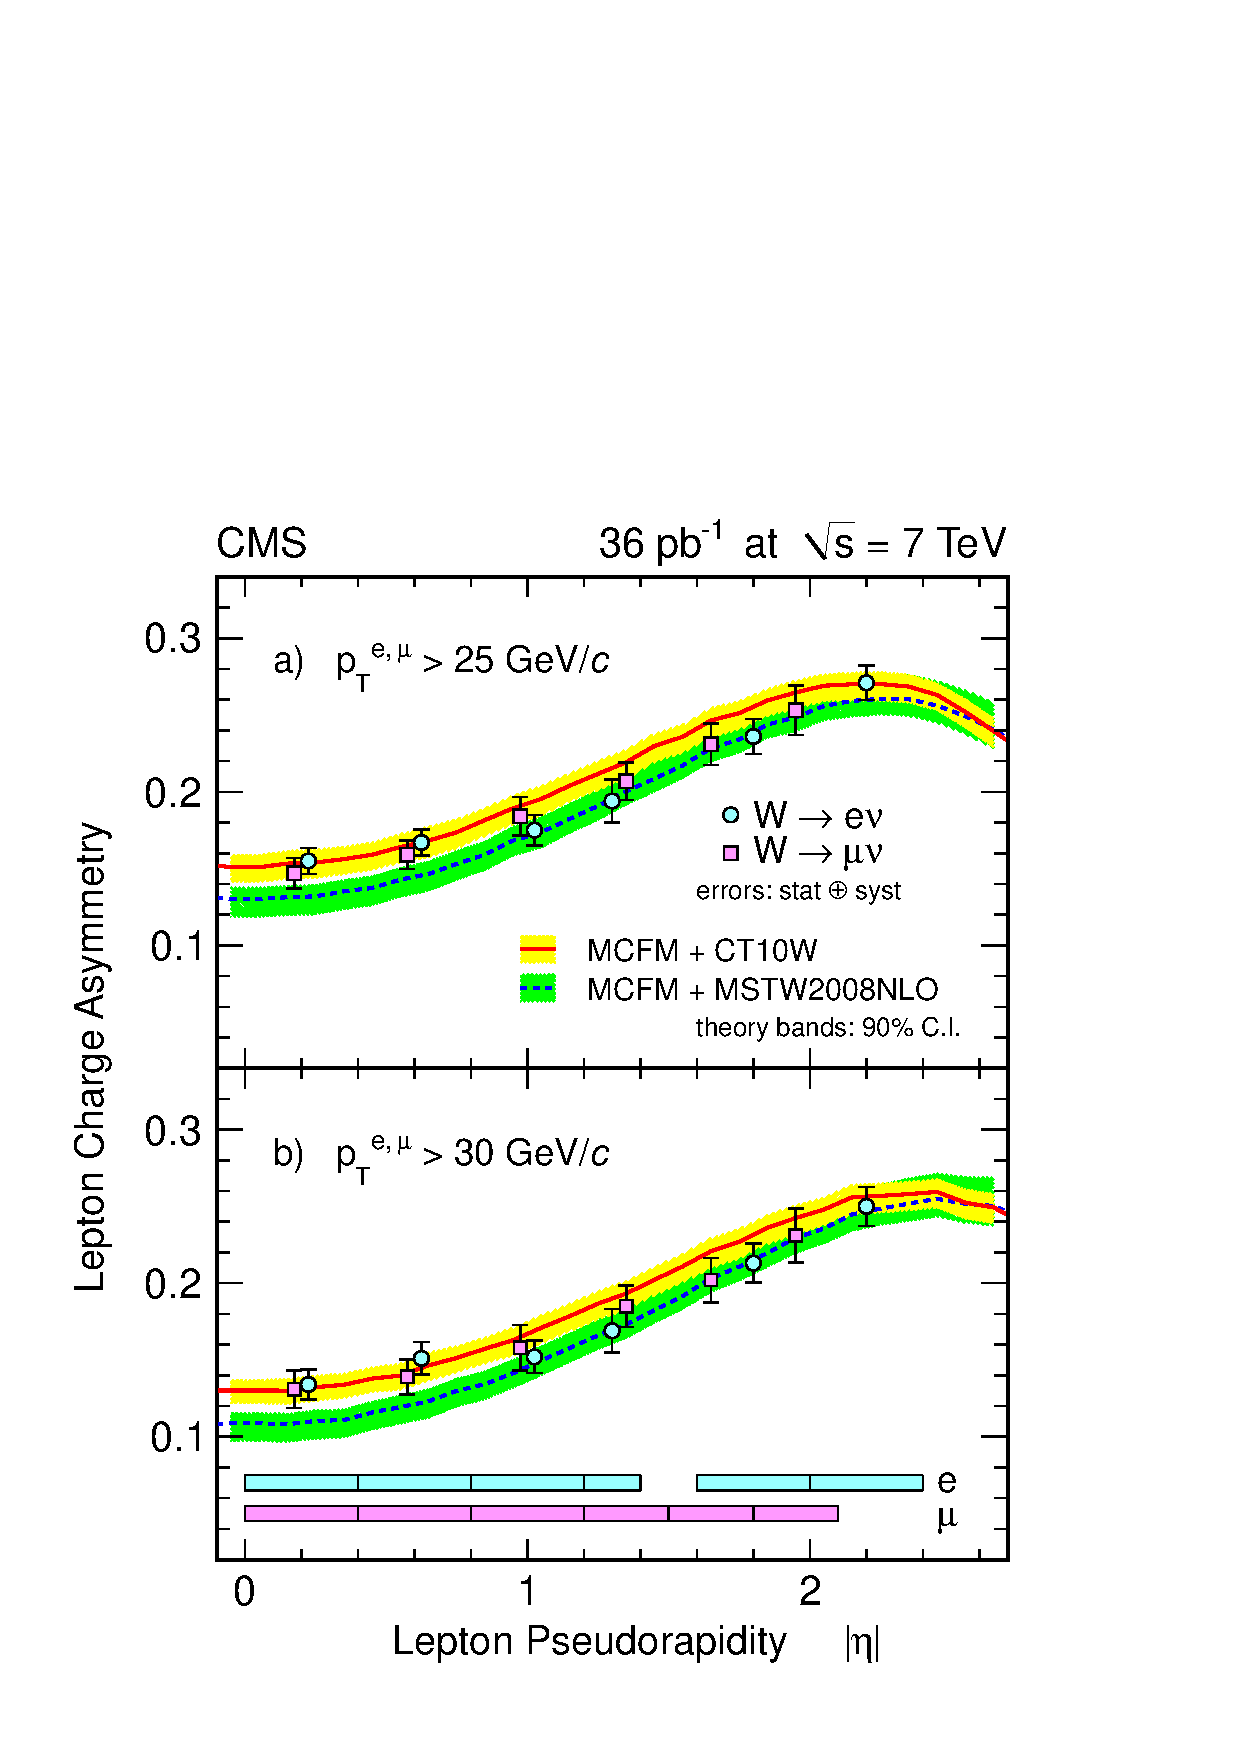
\includegraphics[width=0.80\textwidth]{5-LHCdata/figs/fig2.pdf}
\caption[CMS 2010 $W$ asymmetry data]{CMS 2010 $W$ asymmetry data from the electron and muon decay channels. Figure from ~\cite{Chatrchyan:2011jz}. The figure demonstrates the good agreement of the CT10 PDF set with the experimental data, and the somewhat poorer agreement of the MSTW2008 set, a typical feature of the MSTW fit with LHC electroweak data.}
\label{fig:CMS2010WASY}
\end{figure}

ATLAS initially published a study of the $W$ muon asymmetry distribution with $31$ pb$^{-1}$ of $7$ TeV data~\cite{Aad:2011yna}. This was followed by studies of the $Z$~\cite{Aad:2011gj} and $W$~\cite{Aad:2011fp}  $p_T$ distributions. The most recent data is provided by a combined study of the $W$ and $Z$ $p_T$ distributions based upon the full 2010 dataset~\cite{Aad:2011dm}.

The LHCb detector has a window upon electroweak vector boson production in the very forward region, a kinematic regime that cannot be explored by the general-purpose detectors. $W$ and $Z$ to muon production data based upon an integrated luminosity sample $37$pb$^{-1}$ was published in Ref.~\cite{Aaij:2012vn}, where data was taken in the pseudorapidity range $2.0 < |\eta| < 4.5$ and presented differentially in the (pseudo)rapidity of the detected lepton (pair). Figure~\ref{fig:LHCBWZ} shows the main result of the LHCb $W/Z$ study and demonstrates the good agreement of the theoretical predictions, within the limited statistical precision available in the forward data sample.

\begin{figure}[ht]
\centering
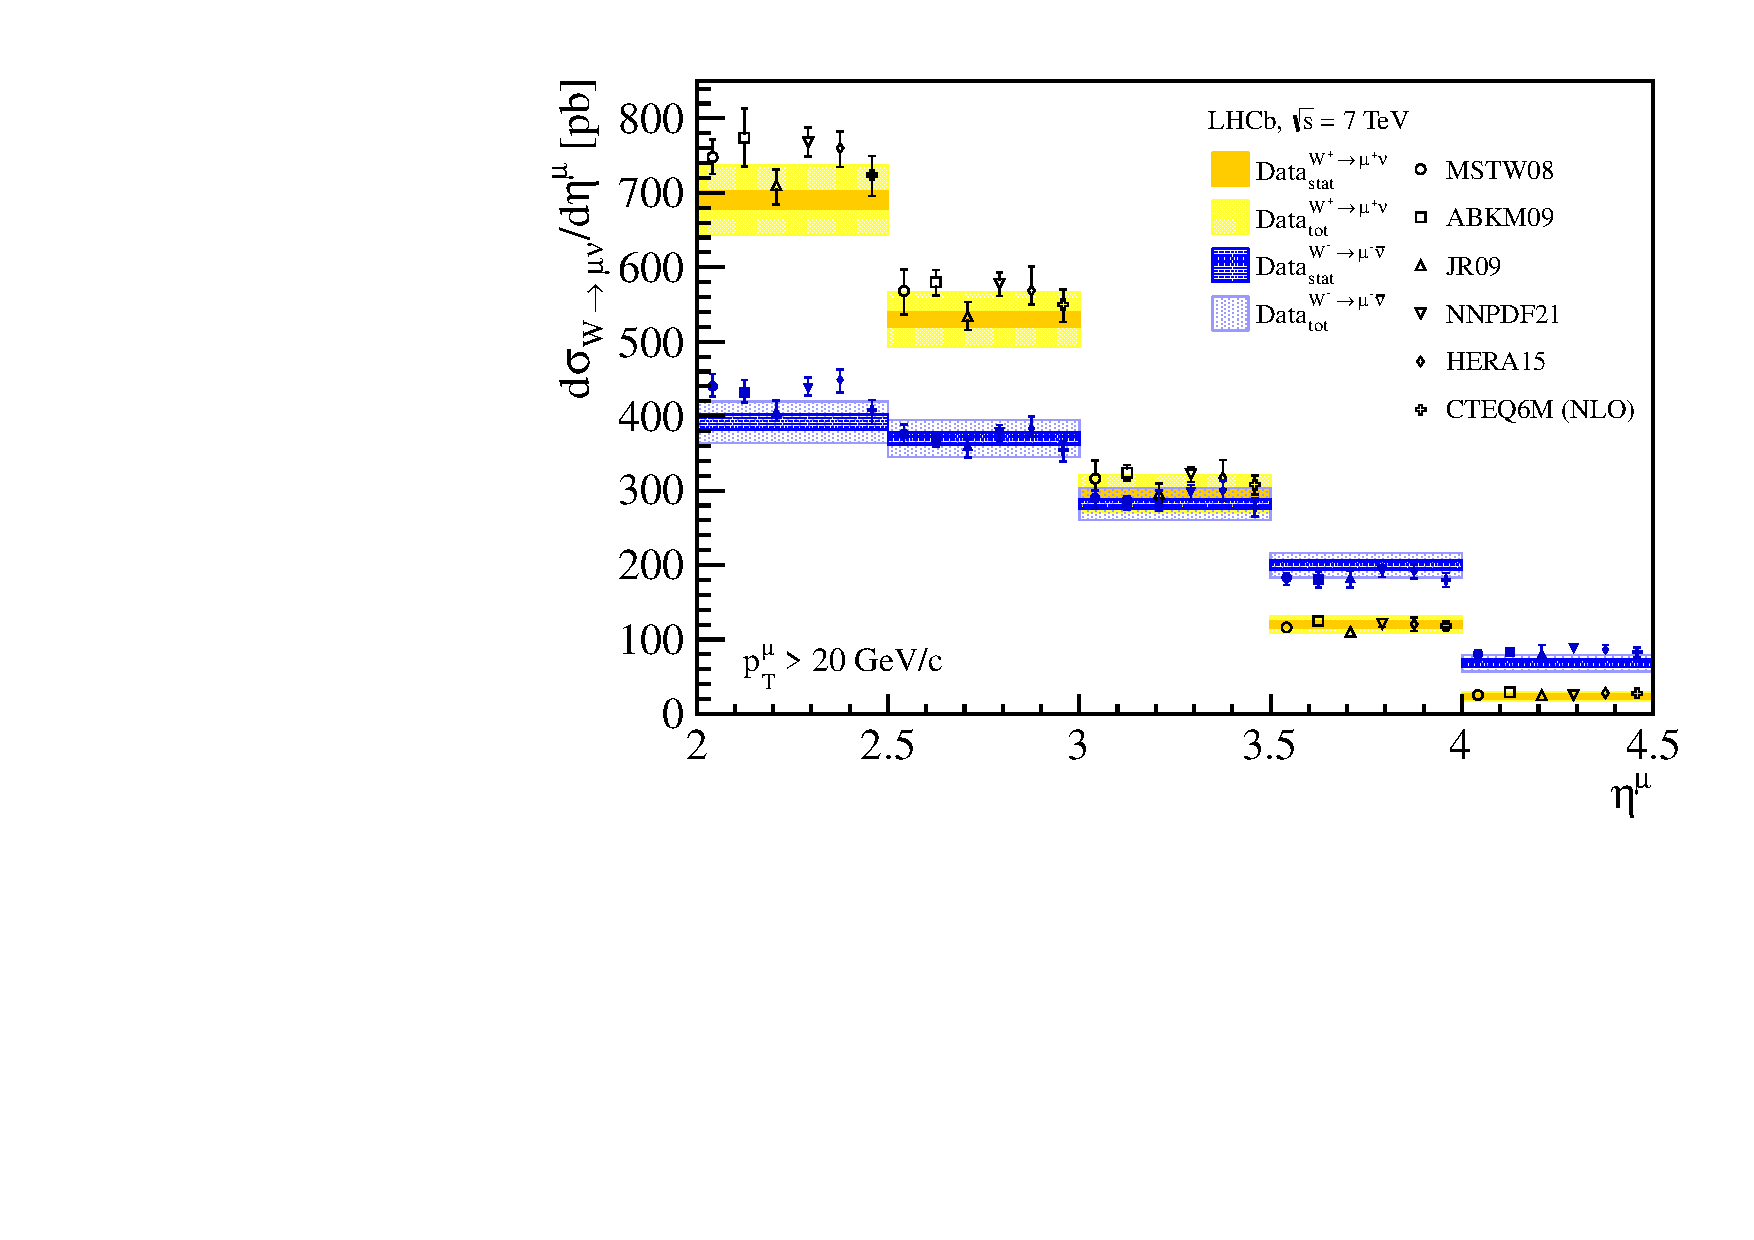
\includegraphics[width=0.48\textwidth]{5-LHCdata/figs/CSW20.pdf}
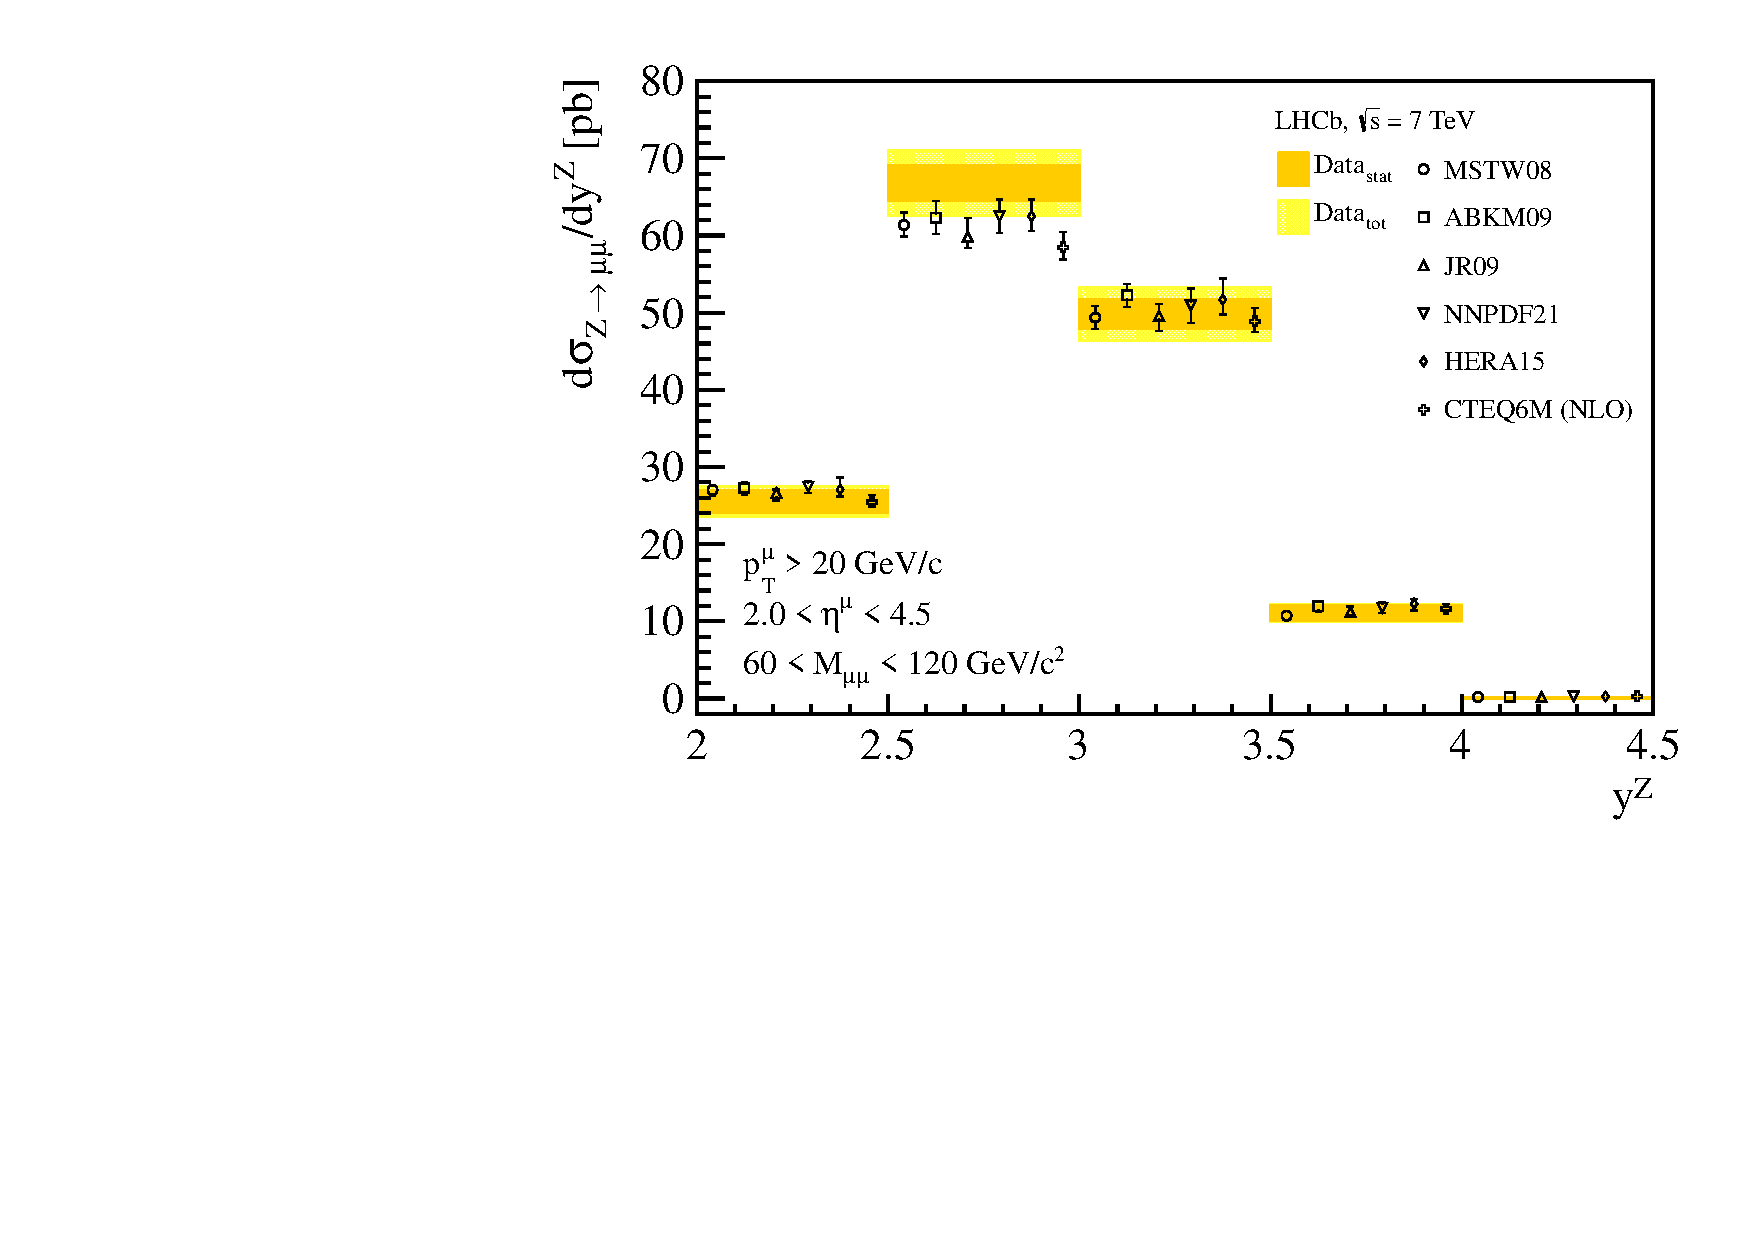
\includegraphics[width=0.48\textwidth]{5-LHCdata/figs/CSZ.pdf}
\caption[LHCb $W$/$Z$ boson (pseudo)rapidity data]{LHCb $W$/$Z$ boson (pseudo)rapidity data. The left panel shows the $W^{\pm}$ distributions in the pseudorapidity of the detected lepton compared to leading PDF sets. The right panel shows the $Z$ in the rapidity of the resulting lepton pair. Figures from~\cite{Aaij:2012vn}.}
\label{fig:LHCBWZ}
\end{figure}

%\subsubsection{Drell-Yan}
%2011 CMS differential in invariant mass Drell-Yan \cite{CMS:2011dxa}
%2011 CMS double differential Y M DY \cite{CMS:2012xxs}
%

\section{Prompt photon data}

Constraints upon the gluon distribution are possible through measurements made of direct photon production at the LHC. Both CMS and ATLAS have published prompt photon data. ATLAS provides inclusive data in photon pseudorapidity intervals of $|\eta| <1.37$ and $1.52 \le |\eta| < 2.37$, for transverse energies $45 \le E_T < 400$ GeV~\cite{Aad:2011tw}, the data showing excellent agreement with predictions from CTEQ6.6 and JETPHOX. Additionally data is available for isolated prompt photon data in association with a jet, based upon the same dataset~\cite{ATLAS:2012ar}, where once again NLO predictions provide a good description of the data, albeit with a small discrepancy arising for photons with $E_T < 45$ GeV.

CMS has performed an isolated photon measurement based upon the same 2010 data run, in the pseudorapidity range $|\eta| < 2.3$ for photons with $25 < E_T < 400$ GeV~\cite{Chatrchyan:2011ue}. The CMS result is plotted in Figure~\ref{fig:CMSpromptphoton}, which shows the agreement between the NLO calculation and the experimental data. The figure demonstrates clearly the precision available of the experimental measurement, however the theoretical predictions clearly suffer from relatively large scale uncertainties. The inclusion of such data into PDF determinations is therefore likely to be challenging without further theoretical progress.

\begin{figure}[ht]
\centering
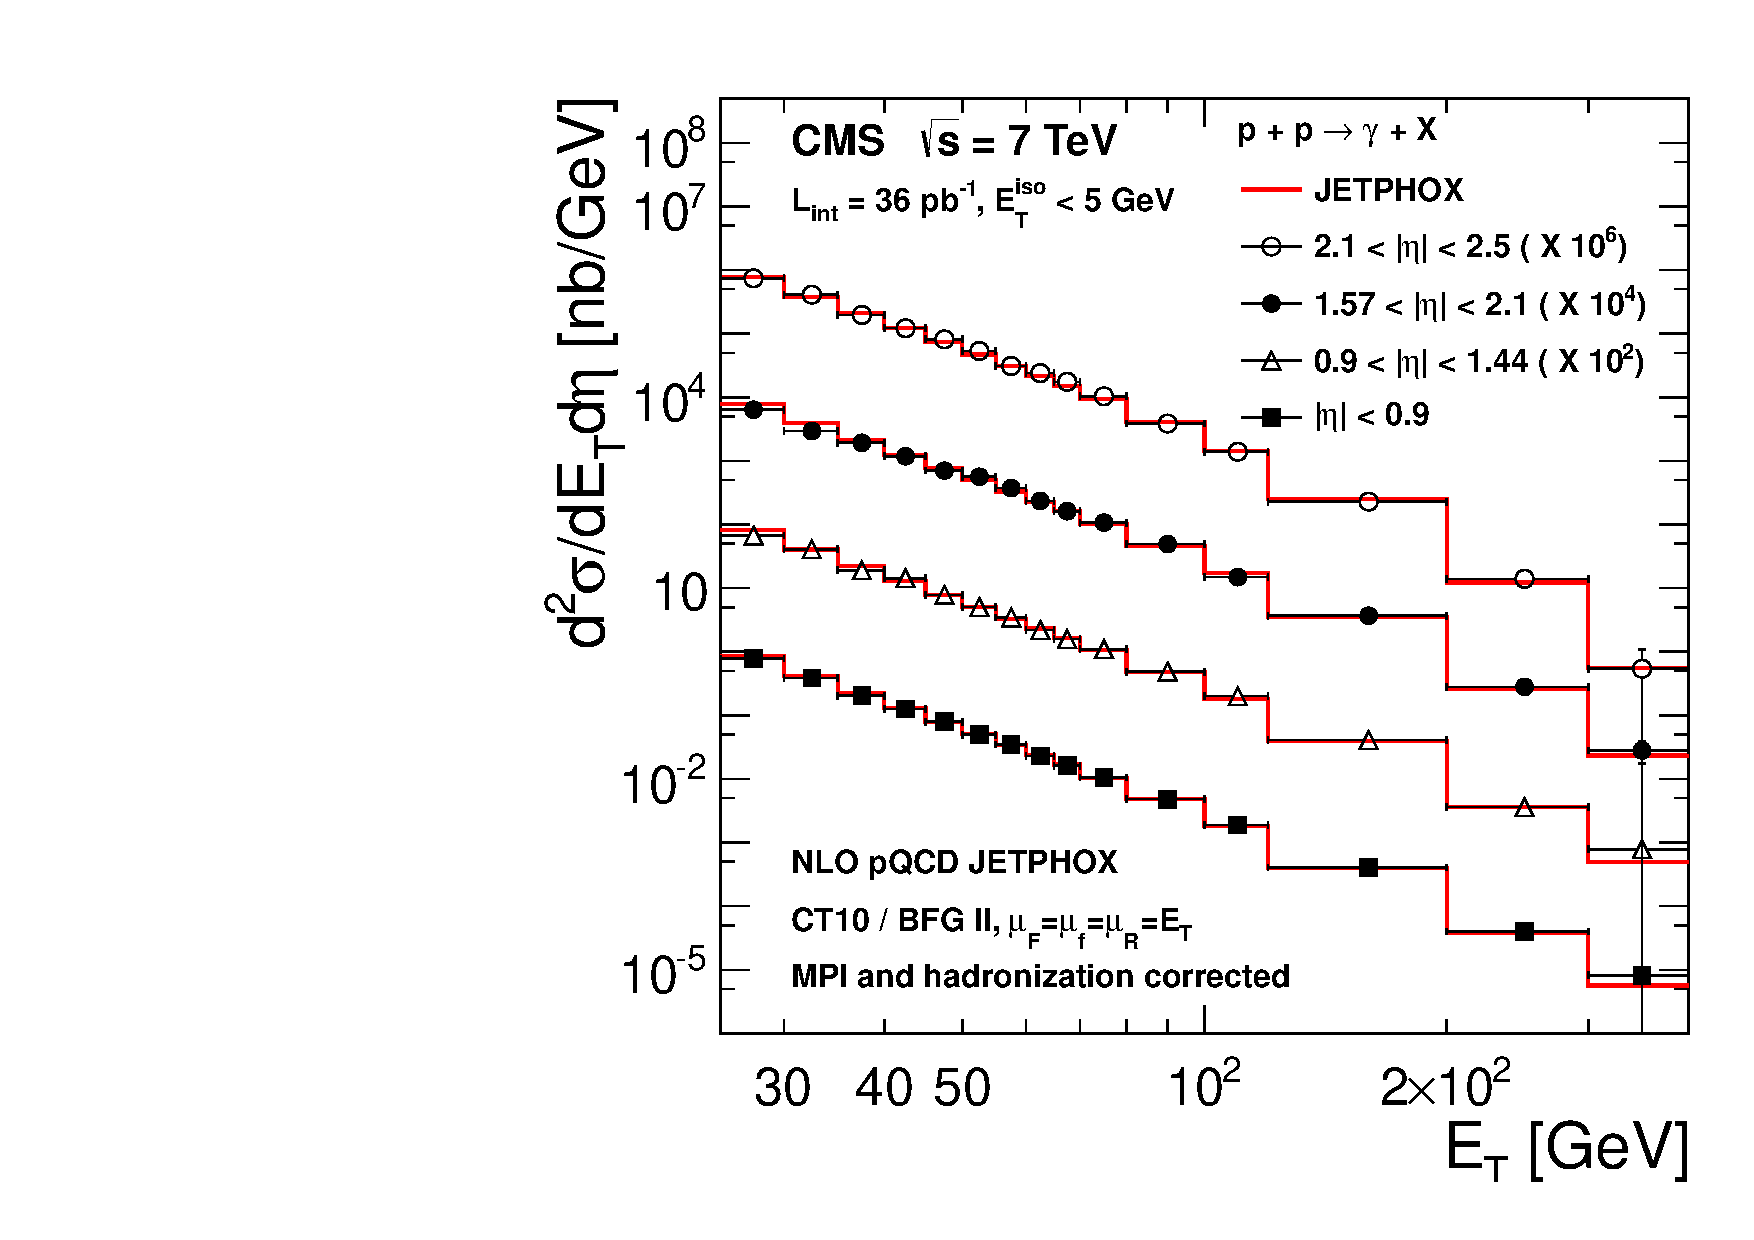
\includegraphics[width=0.48\textwidth]{5-LHCdata/figs/xs_ct10_data_add.pdf}
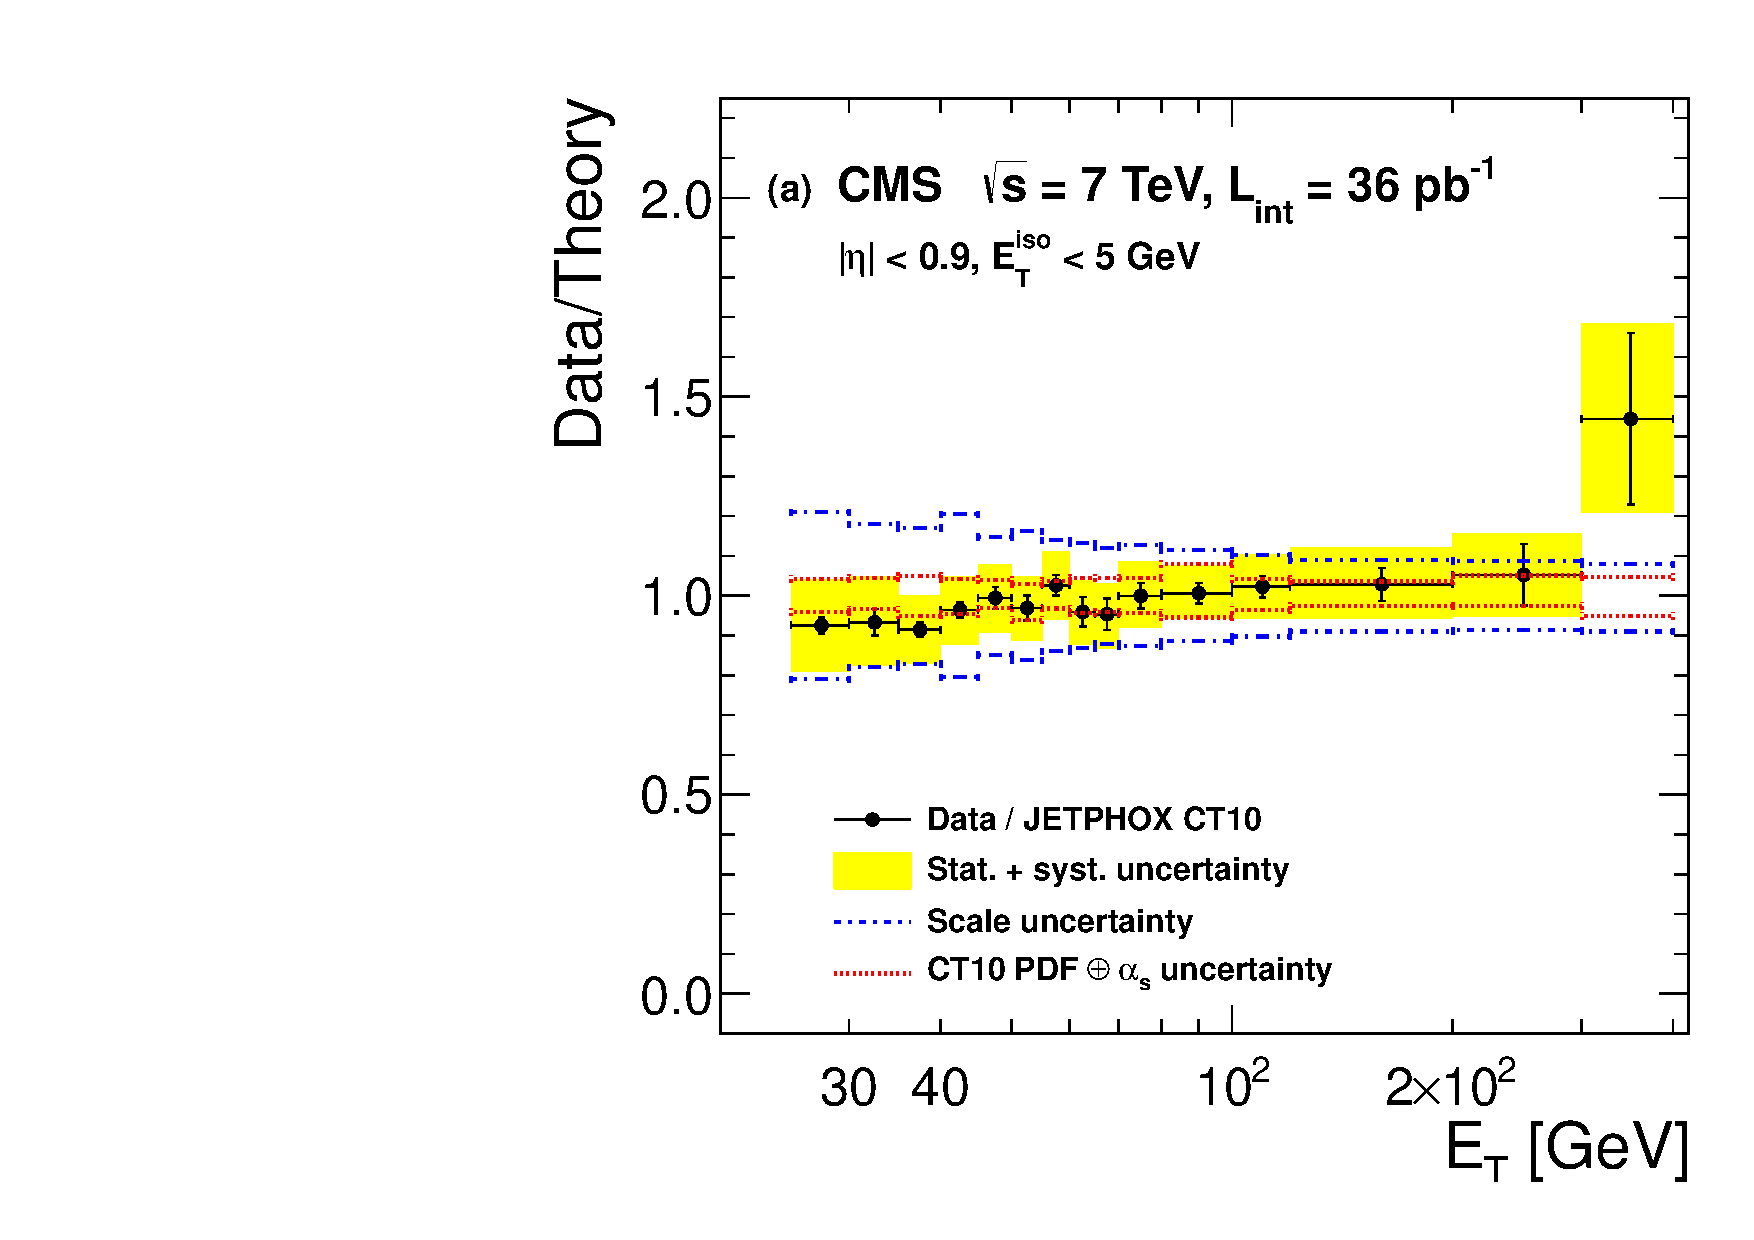
\includegraphics[width=0.48\textwidth]{5-LHCdata/figs/xs_ct10_data_ratio_eta1.pdf}
\caption[CMS isolated prompt photon measurement]{Figures from the CMS isolated prompt photon measurement~\cite{Chatrchyan:2011ue}. The left panel shows the full dataset compared to the CT10/JETPHOX predictions. The right panel shows the result for the lowest pseudorapidity bin as a ratio to the CT10 central value.}
\label{fig:CMSpromptphoton}
\end{figure}

\section{Top pair production data}
LHC collaborations have made extensive measurements of the top pair production cross-section, building upon the combined Tevatron analysis of~\cite{Aaltonen:2012ttbar}. Unlike at the Tevatron where the $qq$ initiated channel is favoured, $t\bar{t}$ data at the LHC is primarily a probe of the gluon content of the proton through the $gg \to t\bar{t}$ subprocess.
The ATLAS collaboration has published measurements of the $t\bar{t}$ cross section in a number of channels, with combination results available at both $7$ TeV~\cite{ATLAS:2012jyc} and $8$ TeV ~\cite{ATLAS:2012fja} centre of mass energies. Likewise CMS have published combined $t\bar{t}$ analyses at $7$~\cite{Chatrchyan:2012bra} and $8$~\cite{CMS:2012iba} TeV. These results are compared to the theoretical prediction obtained from NNPDF2.3 at NNLO+NNLL with { \tt top++ v2.0}~\cite{Czakon:2011xx} in Figure~\ref{fig:LHCttbar}.

\begin{figure}[!]
\centering
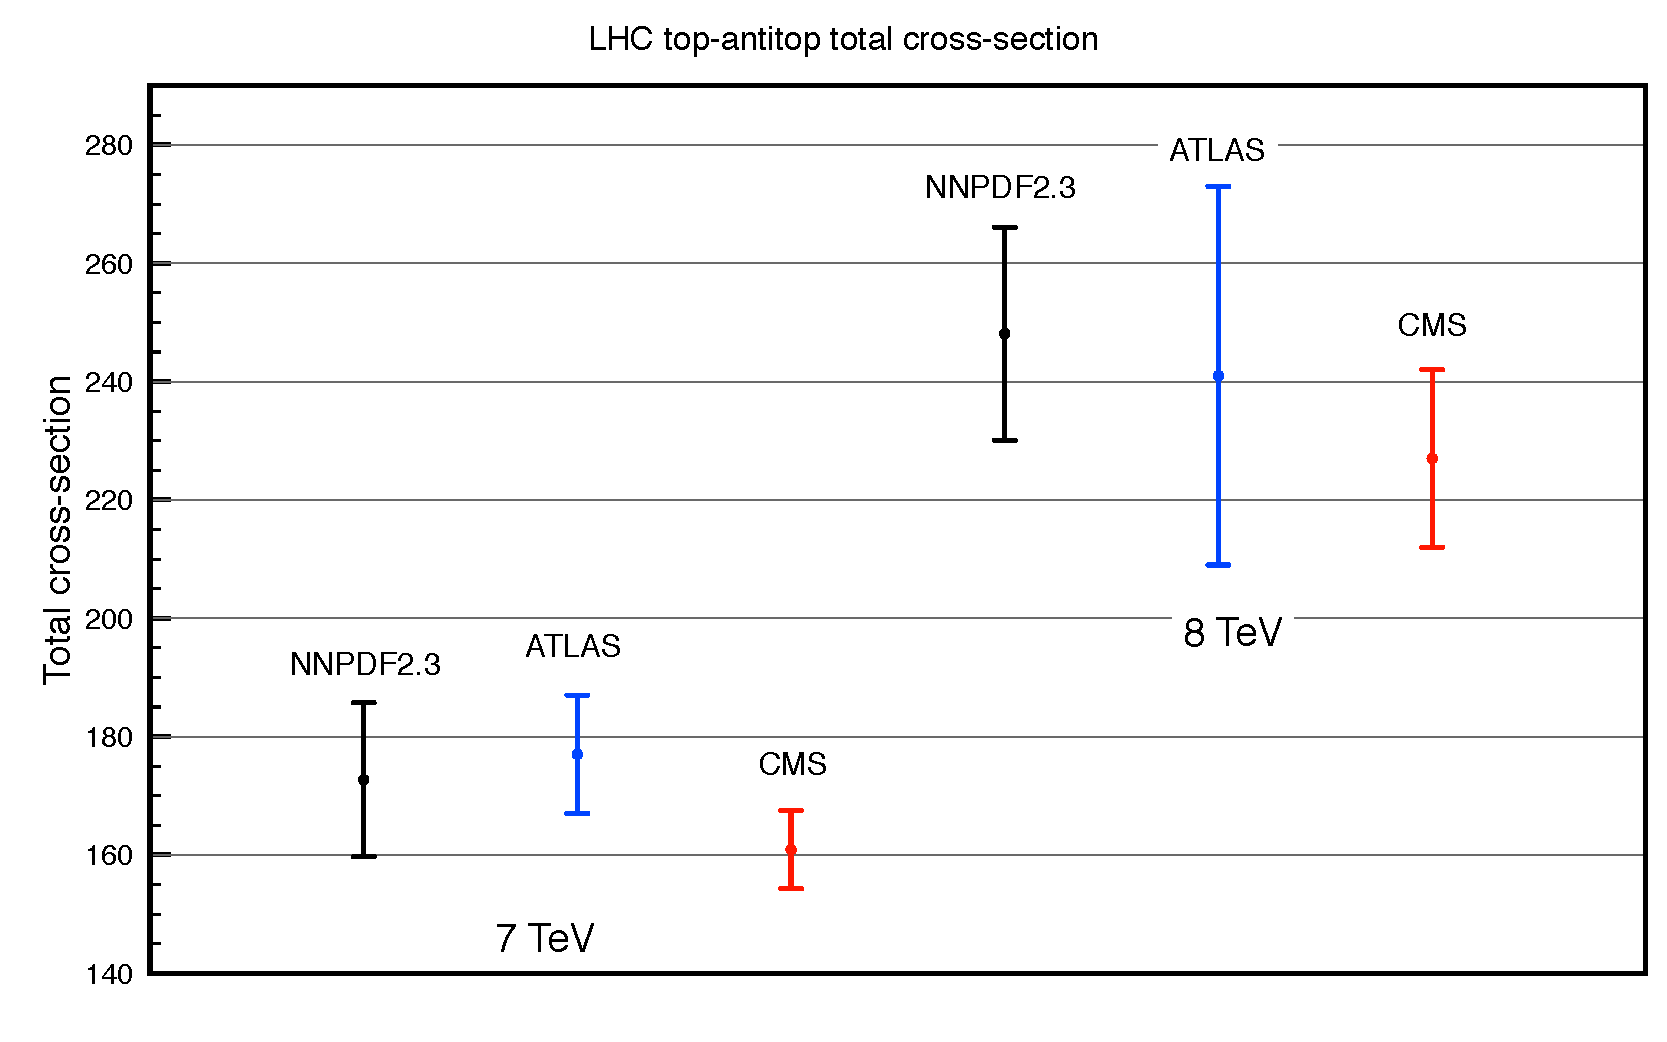
\includegraphics[width=0.8\textwidth]{5-LHCdata/figs/ttbar.pdf}
\caption[LHC 7 and 8 TeV $t\bar{t}$ total cross-section data and predictions from NNPDF2.3]{LHC 7 and 8 TeV $t\bar{t}$ total cross-section data and predictions from NNPDF2.3 at NNLO+NNLL precision. Values in the figure are taken from~\cite{Czakon:2013tha}.}
\label{fig:LHCttbar}
\end{figure}

